
\chapter{Supplementary figures and tables}

\begin{table}[htpb]
\caption{The coordinates of the locations for where the FLEXPART backward simulations are initiated}
\centering
\label{tab:coordinates_clp}
\begin{tabular}{@{}lll@{}}
\toprule
 & Longitude & Latitude \\ \midrule
SACOL & 104.137 & 35.964 \\
Shapotou  & 105.0475 & 37.749  \\
Yinchuan & 106.101 & 38.50 \\
Lingtai & 107.789 &  35.710\\
Lantian & 109.256 & 34.18 \\
Luochuan & 109.424 &  35.710\\
Badoe & 111.17  &  39.003  \\ \bottomrule
\end{tabular}
\end{table}

\begin{figure}[htbp]
    \centering
    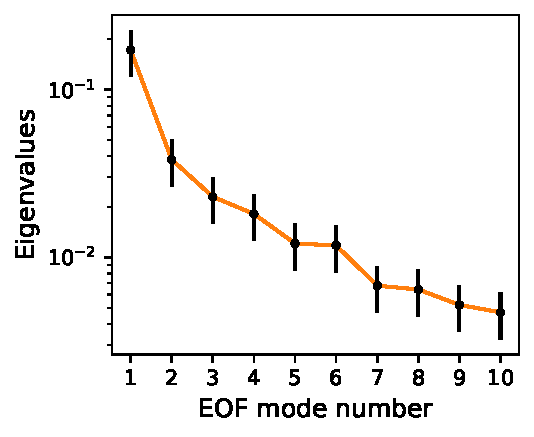
\includegraphics[scale=0.8]{texfiles/figs/EOF_north_test.pdf}
    \caption{The eigenvalues of the 10 first leading EOFs. The error bars correspond to the typical error of each EOF}
    \label{fig:eof_test}
\end{figure}


